The parallel implementation for PFEM-2 follows the guidelines presented by Gimenez et. al. in \cite{gimenez:parallel} for the case of distributed memory architectures. The challenges of serial implementations are well described by Gimenez et. al. and basically involves the extra amount of memory needed for the particle data structure. Due to the explicit scheme the parallel implementation needs to take care of local operations for each particle separately from the rest allowing for a relatively simple parallelization. The difficulty arise at the interface between processors where particles may travel several elements and possible processors before finding their final host element. This task requires an outer loop to communicate particles among processors. This loop will terminate when no more particles cross the interface between partitions. In Fig. \ref{fig:parallel} there is an illustration of how particles may move across processors. The thick black line depicts the partition. In the first case a particle lands in the same processor which involves no communication. In the second case a particle moves across a single interface and communication takes place. In the third place a particle may move across two or more processors in which case the outer loop will perform as many communications as necessary until no more particles cross a processor interface.
%
\begin{figure}[htp] 
\centering 
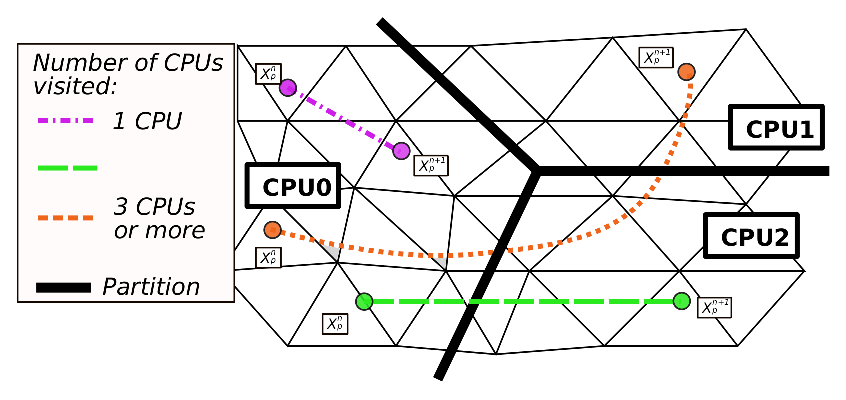
\includegraphics[scale=.6]{./imgs/parallel.eps}
\caption{Different ways that particles may move across processor interfaces.}
\label{fig:parallel}
\end{figure}
%
The current approach is built ``on top'' of a pre-existing parallel FEM implementation thus inheriting much of the data structures and methodologies where the partitions are created using the software METIS \cite{metis1,metis}.

In the present implementation load balancing has not being addressed. Strictly speaking if particles are not removed from the domain then accumulation of particles in one partition will be an issue. As mentioned before the idea of this paper is to evaluate PFEM-2 without introducing the error associated to the removal of particles. A future implementation will tackle this issue. The techniques for particle inventory presented in \cite{gimenez-difusion} will be a good starting point for the implementation.

To exemplify scalability a 3D problem of the flow past a cylinder is used. It has a relatively small number of elements (of about 200 thousand) compared to the element numbers used in the application examples. 
In Fig. \ref{fig:scalab} the strong scalability of the full formulation (FEM+PFEM-2) is shown for distributed memory parallelization. There are two curves for two different inventory strategies. To show the advantages and importance of implementing a particle inventory strategy that is able to remove particles in the first case the number of particles is kept constant at each element regardless of the accuracy of the result. The total number of particles in this case is around 5.7M. In the second case the number of particles changes. No particle is removed from the model except for those that leave the domain and particles are added in elements with less than 12 particles. So the total number of particles is expected to increase as shown in Fig. \ref{fig:cyl_npart}. The final number reaches about 30M particles. Since there is no load balancing particles that accumulate in an element are expected to degrade the scalability which is what is observed in Fig.~\ref{fig:scalab}. The scalability for the first case compares well with that of \cite{gimenez:parallel}.
%
\begin{figure}[htp] 
\centering 
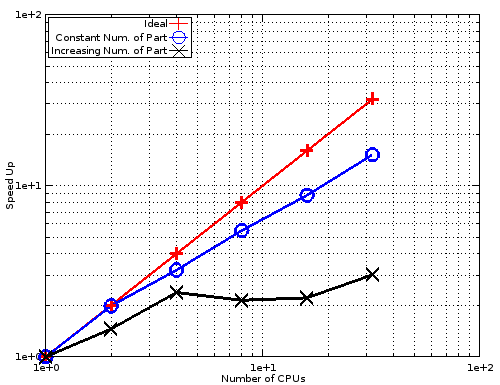
\includegraphics[scale=.6]{./imgs/scalability1.png}
\caption{Comparison of scalability plots for the cases where the number of particles per element is kept constant and the case where no particle removal takes place so the number of particles increase without load balancing.}
\label{fig:scalab}
\end{figure}
